\documentclass{llncs}

\usepackage[margin=1in]{geometry}

\usepackage{graphicx,color,comment,url} 

\usepackage{amsmath,amssymb}


\title{[ML20] Assignment 10}
\author{Your Name}
\institute{}

\begin{document}

\maketitle 

\setlength\parindent{0pt} 
\setlength{\parskip}{10pt}

Due: Apr 20 (b 8:45am) 

Implement K-means algorithm from scratch 
and apply it to cluster the entire data set. 

[1] Visualize your clustering result in a 2D 
feature space obtained by PCA. (You need to 
first cluster instances in the original feature 
space, and then plot their clustering result in 
the 2D space.) 
Mark instances in one cluster by one color, 
and instances in different clusters by different 
colors, e.g., all instances 
in Cluster 1 are red and all in Cluster 2 are blue. 
Choose your own value of K to get a clustering 
result that can be easily explained, 
e.g., if we observe two distant groups of instances 
in the 2D space, but you set K = 1, then it is hard to 
explain why these two groups are assigned to the same 
cluster. 

Figure \ref{hw10_fig1} is an example plot with 
K = 3 on a different data set. You don't have to 
plot cluster centroids,
and your data distribution and clustering result will probably look different from it. 

\begin{figure}[h!] 
\centering 
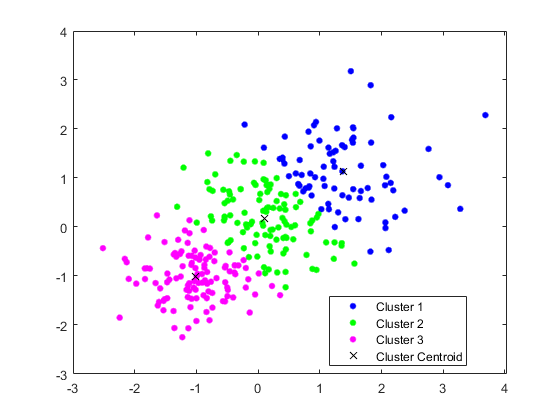
\includegraphics[width=.4\textwidth]{assignment/hw10_fig1.png} 
\caption{Clustering Result of K-means (K = 3).} 
\label{hw10_fig1}
\end{figure}

[2] Choose a proper K so that you can run 
the same algorithm multiple times to obtain 
different clustering results. Show two different 
clustering results in Figure \ref{hw10_fig2} 
and Figure \ref{hw10_fig3}, respectively. 
(Same form as Figure \ref{hw10_fig1}.)

\begin{figure}[h!] 
\centering 
\includegraphics[width=.4\textwidth]{} 
\caption{Clustering Result of Trial 1. 
(K = ...) } 
\label{hw10_fig2}
\end{figure}

\begin{figure}[h!] 
\centering 
\includegraphics[width=.4\textwidth]{} 
\caption{Clustering Result of Trial 2. 
(K = ...) } 
\label{hw10_fig3}
\end{figure}

[3] Vary K to get different clustering result. 
For each result, evaluate its quality using  
two metrics 
\begin{equation}
J_{1} = \frac{1}{K} 
\sum_{k = 1}^{K} \sum_{x_{i} \in C_{k}} 
|| x_{i} - \mu_{k} ||^{2} \qquad 
\text{and} \qquad 
J_{2} = \sum_{k = 1}^{K} \sum_{x_{i} \in C_{k}} 
|| x_{i} - \mu_{k} ||^{2}. 
\end{equation}
Plot two figures. Figure \ref{hw10_fig4} 
shows a curve of $J_{1}$ versus $K$, and 
Figure \ref{hw10_fig5} shows a curve of $J_{2}$ 
versus $K$. (Thus y-axis is $J$ and x-axis is $K$.) 
Choose 7 values of $K$ by yourself for both figures,
and try to cover the behaviors of $J_{1}$ and
$J_{2}$ as comprehensive 
as possible. (Think about how $J$ will behave 
as $K$ decreases and increases.)


\begin{figure}[h!] 
\centering 
\includegraphics[width=.6\textwidth]{} 
\caption{Clustering Quality 
$J_{1}$ versus K.} 
\label{hw10_fig4}
\end{figure}

\begin{figure}[h!] 
\centering 
\includegraphics[width=.6\textwidth]{} 
\caption{Clustering Quality $J_{2}$ versus K.} 
\label{hw10_fig5}
\end{figure}

[4] Apply GMM to cluster the same data set 
and visualize your result in Figure \ref{hw10_fig6}. 
(Same form as Figure \ref{hw10_fig1}.) 
No need to implement GMM from scratch -- just 
use any GMM library. Use the same K as in task 
[1]. (Compare this result with your 
K-means clustering result by yourself.) 

\begin{figure}[h!] 
\centering 
\includegraphics[width=.6\textwidth]{} 
\caption{Clustering Result of GMM. (K = ...)} 
\label{hw10_fig6}
\end{figure}
\end{document}

